\section{Classic methods}
The field of Medical Image Analysis originated from Computer Vision in the early 1990s. Researchers with CV background started applying already established mathematical methods to medical images. In 1996 this newly emerging field got its own archival journal \textit{Medical Image Analysis}. To this day, it is a leading medium that publishes new research results from this area \cite{wells2016}.

In this section I would like to focus on fundamental approaches for image segmentation used at the beginnings. Segmentation is a process of separating objects from the background or from other objects. We can do this by identifying every pixel that belongs to this object or finding its boundaries. In the medical field, segmentation can be used for automated classification of blood cells, detection of tumors, measuring tumor volume and its response to therapy and many more.

\subsection{Thresholding}
Thresholding \cite{thresholding} is a technique based on finding a grey level -- threshold \textit{T}. Every pixel value is compared to this threshold and then assigned to either object or background. Suppose we have an image or its part \textit{f(x,y)}. The thresholded image \textit{g(x,y)} is defined as:

\begin{equation}
    g(x,y) = 
    \left\{\begin{matrix}
    1  &  if (x,y) > T \\ 
    0  &  if (x,y) \leq T
    \end{matrix}\right.
\end{equation}

If the histogram of our image is bimodal (a histogram with two separated peaks), we can assume its peaks represent an object and a background. In this case, we can use one threshold for the whole image. This is called \textit{global} thresholding. 

The global threshold can be chosen manually -- by looking at the histogram and choosing the grey level value at the bottom of the valley separating the peaks. There are also methods to automatise this process. Otzu's method finds the threshold that minimizes intra-class variance, which he shows is the same as maximizing inter-class variance \cite{otzu1979}.  

\textit{Global} thresholding does not always provide sufficient results. If the object has various intensity values, isn't on a contrasting background or is noisy, a different method has to be used. One of the solutions is \textit{local (adaptive)} thresholding. The image is divided into overlapping rectangular regions. A histogram is computed for each of these subimages and then the threshold for this region is chosen. This method is computationally more demanding than finding a \textit{global} threshold. 

Medical images are often blurry, noisy, with low contrast. Histrograms of such images are not bimodal, which causes problems with finding the right threshold. Some pre-processing techniques can help in such situations. We can try to smooth out the edges using various filters. Filters usually have a NxN shape, where N = 3, 5, 7, etc. 

One of the filters is \textit{mean} filter. For every pixel in the picture we find the average of the pixels in its local neighbourhood and that is its new value. Another common filter is \textit{median} filter, which computes the median value for for the neighbouring region. These filters change the histogram in a way that makes it possible to select the threshold. 

\subsection{Region Growing}
The region growing method \cite{medical-imaging-handbook}, as opposed to thresholding, is based on finding connected regions of pixels with similar values. The first step of the algorithm is to select one or more seeds -- pixels that belong to the object. 

The next step is checking all neighbouring pixels, whether they are similar enough to be added to the growing region. The similarity criterion is called uniformity test. This algorithm continues until there are no more pixels that can be added to the region. All the pixels that have been added to the region represent the object. 

The choice of the uniformity test is crucial, the result of region growing is heavily dependant on it. One of the tests can be to compare a pixel value to the mean of the already found region. A threshold for accepting pixels needs to be set. If the difference between the value and the mean is smaller than the threshold, the pixel is added to the region.

Region growing is a very simple technique. It can segment objects with predefined properties. It is computationally not demanding, as it visits every pixel a limited amount of times. On the other hand, it is very sensitive to noise.


\subsection{Watershed Algorithm}
Another region-based method is watershed algorithm \cite{medical-imaging-handbook}. This process can be viewed as filling valleys with water. 

First, seeds for the algorithm need to be chosen. Every object in the image, including the background, needs to be marked by a seed. These can be chosen by an expert or by some automated algorithm specific for the given domain.

We can look at the image as if it were a topographic map. Dark pixels represent valleys, bright ones represent mountaintops. The seeds represent holes in the valleys. Through these holes, water is flowing into their respecting valleys. At one point, waters from two different `lakes' meet. This is where we build a dam -- a border between two objects in the picture.

\subsection{Edge-based Segmentation Techniques}
Locating edges of objects is another way to segment images \cite{medical-imaging-handbook}. Edges in a picture \textit{f(x,y)} are defined by the local intensity gradient. Gradients approximate the first-order derivative of the image-function. The magnitude of a gradient can be calculated as

\begin{equation}
\label{eq:magnitude}
    \left | G \right | = \sqrt{ \left [ {G_{x}}^{2} + {G_{y}}^{2} \right ] } = \sqrt{\left [ \left ( \frac{\partial f}{\partial x}  \right )^{2} \right ] + 
\left [ \left ( \frac{\partial f}{\partial y}  \right )^{2} \right ]
}
\end{equation}

where \textit{$G_{x}$} is a gradient in the \textit{x} direction and \textit{$G_y$} is a gradient in the \textit{y} direction. We can look at them as gradients in the horizontal and vertical directions. Magnitude can be displayed as an image, where it is proportionally represented by grey level values. 

There are a lot of popular gradient operators to compute approximations of derivatives. They are usually filters that use convolution. Convolution is an operation, that computes weighted summations of values in local neighbourhoods. 

The filters have usually two kernels, so both horizontal and vertical changes can be detected. These gradients are then combined using \ref{eq:magnitude} creating the gradient magnitude image. Some of the filters are:

\textit{Sobel edge operator}
\[ 
\begin{array}{cc}

    \begin{bmatrix}
    -1 & -2 & -1 \\
    0 & 0 & 0 \\
    1 & 2 & 1 
    \end{bmatrix} 
                    
    \begin{bmatrix}
    -1 & 0 & 1 \\
    -2 & 0 & 2 \\
    -1 & 0 & 1
    \end{bmatrix}
    
\end{array}
\]
\pagebreak

\textit{Prewitt operator}

\[ 
\begin{array}{cc}

    \begin{bmatrix}
    1 & 1 & 1 \\
    0 & 0 & 0 \\
    -1 & -1 & -1 
    \end{bmatrix} 

    \begin{bmatrix}
    1 & 0 & -1 \\
    1 & 0 & -1 \\
    1 & 0 & -1
    \end{bmatrix}
    
\end{array}
\]

\textit{Roberts Cross operator}
\[ 
\begin{array}{cc}

    \begin{bmatrix}
    1 & 0 \\
    0 & -1 
    \end{bmatrix} 

    \begin{bmatrix}
    0 & 1 \\
    -1 & 0 
    \end{bmatrix}
    
\end{array}
\]

Gradient operators are often followed by a thresholding operation. In this step it is decided, whether an edge has been found or not. The result of this operation is a binary image containing the detected edges.  

Apart from the first-order derivatives, also the second-order derivatives can be used to detect boundaries of objects. Peaks in the first-order correspond to zeros in the second-order derivatives. \textit{Laplacian operator} is able to approximate them. The operator $\nabla^2$ of an image function \textit{f(x,y)} is defined as:

\begin{equation}
    \nabla^2f(x,y) = \frac{\partial^2 f(x,y)}{\partial x^2} + 
    \frac{\partial^2 f(x,y)}{\partial y^2}
\end{equation}

Convolutional masks that approximate \textit{Laplacian operator} can be:

\[ 
\begin{array}{cc}

    \begin{bmatrix}
    0 & -1 & 0 \\
    -1 & 4 & -1 \\
    0 & -1 & 0 
    \end{bmatrix} 

    \begin{bmatrix}
    -1 & -1 & -1 \\
    -1 & 8 & -1 \\
    -1 & -1 & -1
    \end{bmatrix}
    
    \begin{bmatrix}
    1 & -2 & 1 \\
    -2 & 4 & -2 \\
    1 & -2 & 1
    \end{bmatrix}
    
\end{array}
\]

After applying \textit{Laplacian operator}, edges need to be located. Those are pixels where \textit{Laplacian} passes through zero (pixels, where the operator changes signs). This occurs when the pixel intensity changes rapidly.

\subsection{K-Means Clustering}
Clustering in general is a term which describes a problem of finding groups among a set of objects. These groups are called clusters. Clustering works with unlabeled objects and the goal is to find some categories data is organised into.

There are many ways for describing a cluster \cite{clustering}: The easiest way to understand what a cluster is, is to look at it as a group of objects, where all the objects are similar to each other. Moreover, objects in two different clusters should be different. From a more analytical point of view, objects can be seen as points in a space where we can measure distance between them. Any two points in one cluster should be closer to each other than two points from different clusters. Furthermore, clusters should be regions with high-density of points, separated by regions of low-density.

Clustering is used in machine learning as a means to find unknown patterns in n-dimensional data. It is considered unsupervised learning, since it takes unlabeled data as its input, and outputs data separated into categories. 

One of the most popular algorithms for solving the clustering problem is K-Means proposed in 1967 \cite{macqueen1967}. The idea is to find \textit{k} clusters and their centroids in a way, that the distance between data points and their assigned cluster centroid is minimised. The \textit{k} is defined by user. In general, the goal is to minimise the objective function:

\begin{equation}
\label{eq:objective-kmeans}
    J = \sum_{j=1}^{k}\sum_{i=1}^{n}\left \| x_{i}^{(j)}-c_{j} \right \|^{2}
\end{equation}

where \textit{J} is the objective function, \textit{k} is the number of clusters and \textit{n} is the number of points within the cluster \textit{j}. $\left \| x_{i}^{(j)}-c_{j} \right \|$ is the distance between a point \textit{x} and a centroid \textit{c} of the cluster \textit{j}.

The way centroids are computed and distances between points are defined, depends on the metric space and operations available. In the Euclidean space the centroid corresponds to the mean of all points in the cluster (as in KMeans). The distance can be Euclidean distance. 

K-Means is an iterative algorithm and consists of the following steps:

\begin{enumerate}
  \item Choose \textit{k} initial cluster centroids
  \item Assign every point in the space to the nearest centroid
  \item Recompute cluster centroids
  \item Repeat steps 2. and 3. until cluster assignments are not changed in comparison to the previous iterations
\end{enumerate}

K-Means is not guaranteed to find the optimal partition, but is widely used for its simplicity. However, the clusters found heavily depend on the initial centroid values. In the original proposal of the algorithm, centroids are initialised randomly.  

This algorithm is used in computer vision and medical imaging for image segmentation as well. Finding clusters in an image is equivalent to assigning a label to every pixel. Resulting segments (clusters) are discrete regions in the image. In case of images, the data points correspond to pixel values \textit{p(x,y)}. In grey-scale images, we have a one-dimensional Euclidean space and for RGB images it is a three-dimensional space. Therefore, clusters contain pixels with similar pixel values, potentially revealing and recognising similar objects in the picture. 

Sometimes it is difficult to see beforehand how many clusters there are in an image. However, for medical images, it is usually known how many clusters some parts consist of. In \ref{fig:kmeans} there are 4 clusters in MRI head image: bone, soft tissue, fat and background \cite{ng2006}.



\begin{figure}[ht]
    \centering
    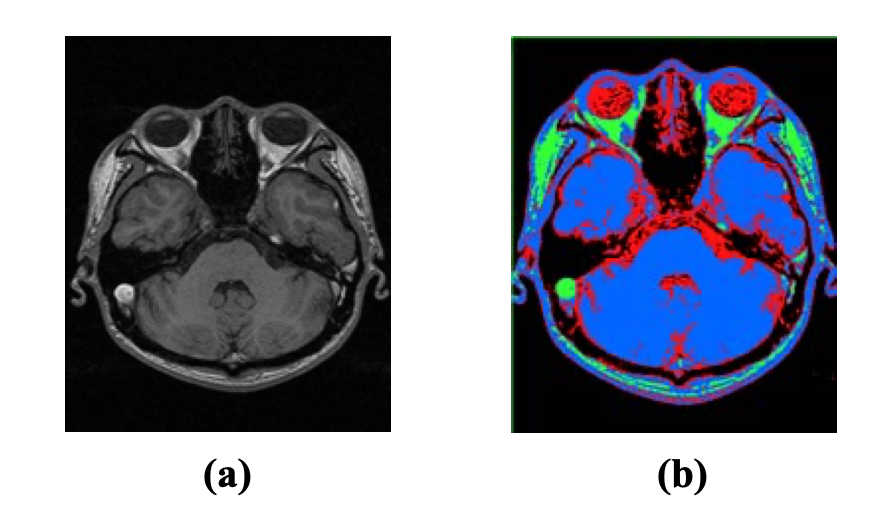
\includegraphics[width=175pt]{images/kmeans.png}
    \caption[K-Means clustering]{Original MRI head image (A) and the image after applying K-Means clustering (B) \cite{ng2006}}
    \label{fig:kmeans}
\end{figure}

\subsection{Fuzzy C-Means clustering}
Fuzzy C-Means clustering \cite{bezdek1981} is another algorithm which aims to solve the clustering problem. It is similar to K-Means as in the number of clusters is set by the user, and it is an iterative algorithm, which loops until some condition is met. 

However, Fuzzy C-Means is based on fuzzy logic. While in K-Means every data point belongs to exactly one cluster, 
in Fuzzy C-Means points can belong to numerous clusters to a certain degree. The membership grade for how strongly they belong to the cluster is between 0 and 1. It is important to point out that these values are not probabilities and do not need to add up to 1.

Fuzziness allows to incorporate uncertainty into our models. To understand what membership means, an example with temperatures is often used. Suppose we want to classify temperatures into groups of \textit{cold}, \textit{warm} and \textit{hot}. It is difficult to determine the threshold between cold and warm or warm and hot, because people perceive these things differently. 

In \ref{fig:fuzzy} the x-axis represents temperature and y-axis membership value. The vertical line is temperature \textit{t}. The membership value for \textit{t} in \textit{cold} is 0.8 which is ``fairly cold''. It is also 0.2 for \textit{warm} which might be interpreted as ``slighty warm''. The membership value for \textit{hot} is equal to 0, so \textit{t} can be considered ``not hot''.  

\begin{figure}[ht]
    \centering
    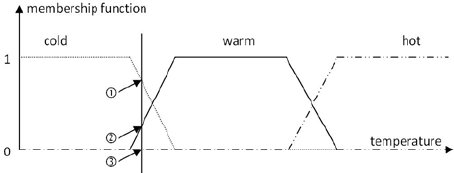
\includegraphics[width=250pt]{images/fuzzy.jpg}
    \caption{Fuzzy logic temperature sets}
    \label{fig:fuzzy}
\end{figure}

Similarly to K-Means, C-Means also aims to minimise an objective function:

\begin{equation}
\label{eq:objective-cmeans}
    J_{m} = \sum_{i=1}^{n}\sum_{j=1}^{c}u_{ij}^{m}\left \| x_{i} - c_{j} \right \|^{2}, 1\leq m\leq \propto 
\end{equation}

where \textit{$J_m$} is the objective function and \textit{m} is a real number which defines how \textit{fuzzy} the clustering should be. \textit{n} is the number of data points and \textit{c} is the number of fuzzy clusters. \textit{$u_{ij}^{m}$} is a membership value for point \textit{$x_i$} in the cluster \textit{$j$}. \textit{$\left \| x_{i} - c_{j} \right \|$} is a distance between a point and the cluster \textit{j} centroid.

The steps for this clustering algorithms are as follows:

\begin{enumerate}
  \item Assign random membership values to all data points for every cluster
  \item Compute the centroid for each cluster:
  
  \begin{equation}
    \label{eq:centroid-cmeans}
    c_{j} = \frac{\sum_{i=1}^{n}u_{ij}^{m} . x^{i}}{\sum_{i=1}^{n}u_{ij}^{m}}
    \end{equation}
    
   \item For each data point, recompute their membership values in the clusters:
   \begin{equation}
    \label{eq:update-cmeans}
    u_{ij} = \frac{1}{\sum_{k=1}^{c}\left ( \frac{\left \| x_i - c_j \right \|}{\left \| x_i - c_k \right \|} \right )^{\frac{2}{m-1}}}
    \end{equation}
    
    \item Repeat steps 2 and 3 until the membership values do not change by more than $\epsilon$, which is a pre-set value between 0 and 1
\end{enumerate}

The output of Fuzzy C-Means Clustering is a list of centroids and a partition matrix \textit{$w_{ij}$}, where each element is the membership value of the data point \textit{$x_i$} in the cluster \textit{$c_j$}. Finally, every point is assigned to the cluster for which it has the highest membership value.

FCM can be used for image segmentation in a similar manner as K-Means. 

